% =====================================================================================
% The Quantum Approximate Optimization Algorithm (QAOA) - from Max-Cut to CUDA-Q
% Build:  python make_figures.py   (needs cudaq, numpy, scipy, matplotlib)
%         latexmk -pdf qaoa_lecture.tex
% Companion of presentations/qft_source/qft_lecture.tex (same layout and colours).
% =====================================================================================
\documentclass[aspectratio=169,11pt]{beamer}
\usepackage[T1]{fontenc}
\usepackage{lmodern}
\usepackage{amsmath,amssymb}
\usepackage{braket}
\usepackage{graphicx}
\usepackage{booktabs}
\usepackage{array}
\usepackage{tikz}
\usetikzlibrary{arrows.meta,positioning,calc}
\usepackage{quantikz}
\usepackage{listings}
\graphicspath{{figures/}}
% GENERATED by make_figures.py - do not edit
\newcommand{\numnedges}{30}
\newcommand{\numcmax}{25}
\newcommand{\numnopt}{4}
\newcommand{\numrandvar}{7.5}
\newcommand{\numrandsd}{2.74}
\newcommand{\numstart}{9.18}
\newcommand{\numstartnp}{9.18}
\newcommand{\numbestcut}{20.5336}
\newcommand{\numratio}{0.8213}
\newcommand{\numnevals}{75}
\newcommand{\numpopt}{0.0600}
\newcommand{\numopthits}{240}
\newcommand{\numeta}{0.553}
\newcommand{\numfid}{1.000000000000}
\newcommand{\numopttime}{70}
\newcommand{\numgammaa}{0.367}
\newcommand{\numgammab}{0.690}
\newcommand{\numbetaa}{1.117}
\newcommand{\numbetab}{-0.275}
\newcommand{\numoptmsg}{Return from COBYLA because the trust region radius reaches its lower bound}
\newcommand{\numshotmean}{20.520}
\newcommand{\numprandopt}{1.22\times10^{-4}}
\newcommand{\numpqaoaopt}{0.0580}
\newcommand{\numtoprows}{\texttt{110010001001101} & 68 & 25\\\texttt{001101110110010} & 67 & 25\\\texttt{110010001011101} & 56 & 25\\\texttt{001101110100010} & 49 & 25\\\texttt{010010001101101} & 40 & 24\\\texttt{101101110010010} & 28 & 24\\}
\newcommand{\numponebest}{18.84}
\newcommand{\numponegamma}{0.47}
\newcommand{\numponebeta}{-0.34}
\newcommand{\numringone}{0.7500}
\newcommand{\numringtwo}{0.8333}
\newcommand{\numringthree}{0.8750}
\newcommand{\numrepoone}{0.754}
\newcommand{\numrepotwo}{0.821}
\newcommand{\numrepothree}{0.861}


% ---- colours and look (identical to the QFT lecture) ---------------------------------
\definecolor{qblue}{HTML}{2A78D6}
\definecolor{qdark}{HTML}{1C5CAB}
\definecolor{qorange}{HTML}{EB6834}
\definecolor{qaqua}{HTML}{1BAF7A}
\definecolor{qink}{HTML}{0B0B0B}
\definecolor{qgrey}{HTML}{52514E}
\definecolor{qlight}{HTML}{EEF4FC}
\setbeamercolor{structure}{fg=qdark}
\setbeamercolor{frametitle}{fg=qdark}
\setbeamercolor{title}{fg=qdark}
\setbeamercolor{normal text}{fg=qink}
\setbeamercolor{block title}{bg=qblue,fg=white}
\setbeamercolor{block body}{bg=qlight,fg=qink}
\setbeamercolor{block title example}{bg=qaqua,fg=white}
\setbeamercolor{block body example}{bg=qaqua!10,fg=qink}
\setbeamercolor{block title alerted}{bg=qorange,fg=white}
\setbeamercolor{block body alerted}{bg=qorange!10,fg=qink}
\setbeamertemplate{blocks}[rounded][shadow=false]
\setbeamertemplate{navigation symbols}{}
\setbeamertemplate{itemize items}[circle]
\setbeamertemplate{enumerate items}[default]
\setbeamerfont{frametitle}{size=\large,series=\bfseries}
% =====================================================================================
% SILICO FELLER branding for the beamer lecture decks (16:9).
% \input this file in the preamble of every presentations/<algorithm>_source/<algorithm>_lecture.tex,
% after graphicx is loaded and the colours/fonts are set. It is the "slide master":
%   * the official logo (assets/branding/silico_feller_logo.png, unmodified, aspect ratio kept)
%     is drawn at the top-right of EVERY slide through the background template, so new or
%     re-ordered slides get it automatically;
%   * the frame-title box is narrowed on the right so titles wrap before they can reach the logo.
% =====================================================================================
\makeatletter
\newcommand{\sflogofile}{../../assets/branding/silico_feller_logo.png}
\newlength{\sflogoheight}\setlength{\sflogoheight}{5.4mm}   % logo height on the slide (width follows the aspect ratio)
\newlength{\sflogomargin}\setlength{\sflogomargin}{2.5mm}   % distance from the top and right paper edges
\newlength{\sflogoreserve}\setlength{\sflogoreserve}{2.6cm} % horizontal space kept free for the logo in the title row

% logo on every slide (background layer: never covers slide content)
\setbeamertemplate{background}{%
  \vbox to \paperheight{%
    \vskip\sflogomargin
    \hbox to \paperwidth{\hfill\includegraphics[height=\sflogoheight]{\sflogofile}\hskip\sflogomargin}%
    \vfill}}

% frame title: same look as beamer's default, but it stops \sflogoreserve before the right edge
\setbeamertemplate{frametitle}{%
  \ifbeamercolorempty[bg]{frametitle}{}{\nointerlineskip}%
  \begin{beamercolorbox}[sep=0.3cm,left,wd=\paperwidth]{frametitle}%
    \usebeamerfont{frametitle}%
    \vbox{}\vskip-1ex%
    \parbox[t]{\dimexpr\paperwidth-0.6cm-\sflogoreserve\relax}{\raggedright
      \strut\insertframetitle\strut\par
      \ifx\insertframesubtitle\@empty\else
        {\usebeamerfont{framesubtitle}\usebeamercolor[fg]{framesubtitle}\insertframesubtitle\strut\par}%
      \fi}%
    \vskip-1ex%
    \vskip-.3cm%
  \end{beamercolorbox}}
\makeatother
   % SILICO FELLER logo on every slide
\setbeamertemplate{footline}{%
  \leavevmode\hbox{\begin{beamercolorbox}[wd=\paperwidth,ht=2.4ex,dp=1ex,leftskip=0.4cm,rightskip=0.4cm]{normal text}%
    \color{qgrey}\tiny The Quantum Approximate Optimization Algorithm\ \ $\cdot$\ \ \insertsectionhead\hfill\insertframenumber\,/\,\inserttotalframenumber
  \end{beamercolorbox}}}
\newcommand{\hl}[1]{{\color{qorange}\textbf{#1}}}
\newcommand{\key}[1]{{\color{qdark}\textbf{#1}}}
\newcommand{\bg}{\boldsymbol\gamma}
\newcommand{\bb}{\boldsymbol\beta}

\lstset{language=Python, basicstyle=\ttfamily\scriptsize, keywordstyle=\color{qdark}\bfseries,
  commentstyle=\color{qgrey}\itshape, stringstyle=\color{qorange}, showstringspaces=false,
  frame=single, rulecolor=\color{qblue!40}, backgroundcolor=\color{qlight}, columns=fullflexible}

\title{The Quantum Approximate Optimization Algorithm}
\subtitle{From Max-Cut to a CUDA-Q implementation --- explained step by step}
\author{CUDA-Q Quantum Algorithm Benchmarking Suite}
\date{Companion lecture to \texttt{QAOA.ipynb}}

\begin{document}

% =====================================================================================
\section{Introduction}
\begin{frame}
  \titlepage
  \centering\small\color{qgrey}
  All quantum results in these slides were computed with NVIDIA CUDA-Q 0.16 (\texttt{qpp-cpu}) using the kernel of
  \texttt{QAOA.ipynb}, and checked against an independent NumPy simulation.
\end{frame}

\begin{frame}{What you will learn today}
  \begin{columns}[T]
    \begin{column}{0.56\textwidth}
      \small
      \begin{enumerate}\itemsep0pt
        \item What an \key{optimization problem} is and why combinatorial ones are hard
        \item Graphs and the \key{Max-Cut} problem
        \item From bits to spins: the \key{cost Hamiltonian}
        \item The qubit toolkit: Pauli operators, rotations, CNOT
        \item The \key{QAOA circuit}: cost layer, mixer layer, depth $p$
        \item The hybrid loop: \key{classical optimizer} + quantum expectation values
        \item Exact analysis at $p = 1$ and worked examples
        \item The CUDA-Q implementation in \texttt{QAOA.ipynb}, line by line
        \item Results, benchmarks, \key{limits}, noise and current research
      \end{enumerate}
    \end{column}
    \begin{column}{0.40\textwidth}
      \begin{block}{You only need}
        \begin{itemize}
          \item school algebra and trigonometry
          \item vectors and matrices
          \item basic probability (averages)
        \end{itemize}
        Everything quantum is explained on the way.
      \end{block}
      \begin{alertblock}{Three kinds of statements}
        \small \textbf{General theory}, \textbf{the notebook's convention}, and \textbf{illustrative
        assumptions} are marked as such.
      \end{alertblock}
    \end{column}
  \end{columns}
\end{frame}

% =====================================================================================
\section{Part 1: Optimization}
\begin{frame}{What is an optimization problem?}
  \begin{block}{Optimization}
    Find the \key{best} element $x^*$ of a set of candidates $\mathcal{X}$ according to an \key{objective function} $f$:
    \[ x^* = \arg\max_{x\in\mathcal{X}} f(x) \qquad(\text{or } \arg\min). \]
  \end{block}
  \begin{columns}[T]
    \begin{column}{0.48\textwidth}
      \key{Continuous}: $x \in \mathbb{R}^d$ --- e.g.\ the best wing shape, the cheapest mixture of materials. Calculus
      (gradients) helps.
    \end{column}
    \begin{column}{0.48\textwidth}
      \key{Combinatorial}: $x$ is a discrete choice --- a route, a schedule, a yes/no per item. No gradients; the
      number of candidates explodes.
    \end{column}
  \end{columns}
  \vspace{2mm}
  Examples from engineering: chip placement, network design, scheduling machines, portfolio selection, clustering data.
\end{frame}

\begin{frame}{Why combinatorial optimization is hard}
  \begin{columns}[c]
    \begin{column}{0.48\textwidth}
      With $n$ yes/no decisions there are $2^n$ candidates:
      \begin{center}\small
      \begin{tabular}{rr}
        \toprule $n$ & $2^n$ candidates\\ \midrule
        10 & 1\,024\\ 15 & 32\,768\\ 30 & $1.1\times10^{9}$\\ 60 & $1.2\times10^{18}$\\ 100 & $1.3\times10^{30}$\\ \bottomrule
      \end{tabular}
      \end{center}
    \end{column}
    \begin{column}{0.48\textwidth}
      \begin{itemize}
        \item Trying all candidates (\key{brute force}) is exact but exponential.
        \item Many such problems are \key{NP-hard}: no polynomial-time exact algorithm is known.
        \item In practice we accept \key{good} answers quickly: heuristics and \key{approximation algorithms} with a
          guaranteed quality.
      \end{itemize}
      \begin{block}{Approximation ratio}
        $r = \dfrac{\text{value found}}{\text{optimal value}} \in [0, 1]$ for maximization.
      \end{block}
    \end{column}
  \end{columns}
\end{frame}

\begin{frame}{Classical tools for combinatorial problems}
  \begin{columns}[T]
    \begin{column}{0.48\textwidth}
      \begin{block}{Exact}
        Brute force ($2^n$), branch and bound, integer programming solvers --- exponential in the worst case.
      \end{block}
      \begin{block}{Heuristics (no guarantee)}
        Greedy local search, simulated annealing, tabu search, genetic algorithms.
      \end{block}
    \end{column}
    \begin{column}{0.48\textwidth}
      \begin{block}{Approximation algorithms (guarantee)}
        For Max-Cut, \key{Goemans--Williamson} (1995): semidefinite relaxation + random rounding gives
        $\mathbb E[C] \ge 0.878\,C_{\max}$ in polynomial time.
      \end{block}
      \begin{exampleblock}{In \texttt{QAOA.ipynb}}
        Exact brute force up to 22 nodes; above that a greedy \emph{local search} with 200 restarts, labelled
        ``NOT guaranteed optimal''.
      \end{exampleblock}
    \end{column}
  \end{columns}
\end{frame}

% =====================================================================================
\section{Part 2: Graphs and Max-Cut}
\begin{frame}{Graph theory in five minutes}
  \begin{columns}[T]
    \begin{column}{0.52\textwidth}
      \begin{itemize}
        \item A \key{graph} $G = (V, E)$: nodes $V = \{0, \dots, n-1\}$ and edges $E \subseteq \{(i,j)\}$.
        \item A \key{weighted} graph gives every edge a number $w_{ij}$; $W = \sum_{(i,j)\in E} w_{ij}$.
        \item \key{Degree} $d_i$ = number of edges at node $i$.
          \textbf{Handshake lemma:} $\sum_i d_i = 2|E|$.
        \item A \key{cycle} returns to its start; it is \key{odd} if it has an odd number of edges.
        \item \key{Bipartite}: nodes can be 2-coloured so that every edge joins different colours $\iff$ no odd cycle.
      \end{itemize}
    \end{column}
    \begin{column}{0.44\textwidth}
      \begin{block}{Standard families}
        \begin{itemize}
          \item ring (cycle) $C_n$: $n$ edges, $d = 2$
          \item complete graph $K_n$: $\binom n2$ edges
          \item random graph $G(n, q)$: each pair is an edge with probability $q$; $\mathbb E|E| = \binom n2 q$
        \end{itemize}
      \end{block}
      The notebook's default: $G(15, 0.3)$ with \texttt{SEED = 42} $\Rightarrow$ \numnedges{} edges (expected $31.5$).
    \end{column}
  \end{columns}
\end{frame}

\begin{frame}{The Max-Cut problem}
  \begin{columns}[c]
    \begin{column}{0.46\textwidth}
      \centering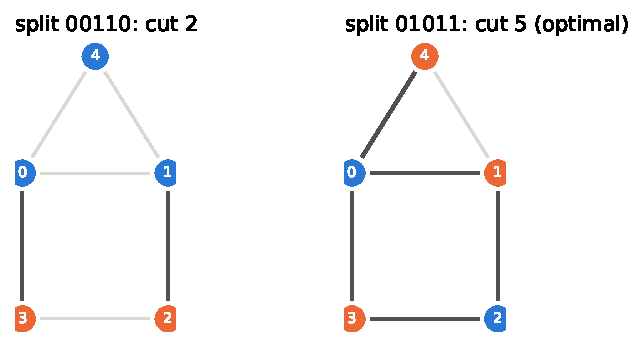
\includegraphics[width=\textwidth]{house}\\
      \small ``House graph'': square $0{-}1{-}2{-}3$ plus roof node 4.
    \end{column}
    \begin{column}{0.52\textwidth}
      \begin{block}{Max-Cut}
        Split the nodes into two groups. The \key{cut} is the total weight of edges \emph{between} the groups. Find the
        split with the largest cut.
      \end{block}
      A split is a bitstring $z = z_0z_1\dots z_{n-1}$, $z_i \in \{0,1\}$ = group of node $i$:
      \[ C(z) = \sum_{(i,j)\in E} w_{ij}\,[z_i \neq z_j] . \]
      $[\,\cdot\,]$ is 1 if the condition holds, else 0. Dark edges in the figure are cut.
    \end{column}
  \end{columns}
\end{frame}

\begin{frame}{Worked example: the house graph}
  \begin{enumerate}
    \item \key{Upper bound.} Nodes $0, 1, 4$ form a triangle (odd cycle): at least one of its edges stays uncut, so
      $C \le 6 - 1 = 5$.
    \item \key{Construction.} Colour the square alternately: $z_0z_1z_2z_3 = 0101$ cuts all 4 square edges. Node 4 sees
      node 0 (group 0) and node 1 (group 1): exactly one roof edge is cut, whatever $z_4$ is. Total $4 + 1 = 5$.
    \item \key{Counting.} $z_0z_1z_2z_3 \in \{0101, 1010\}$ and $z_4$ free: \hl{4 optimal bitstrings}, but only
      \hl{2 different partitions} (a split and its complement $\bar z$ are the same partition).
  \end{enumerate}
  \begin{exampleblock}{Random guessing}
    Each edge is cut with probability $\tfrac12$ by a random split, so $\mathbb E[C] = W/2 = 3$ and
    $r_{\text{random}} = 3/5 = 0.6$. $P(\text{random split is optimal}) = 4/32 = 1/8$.
  \end{exampleblock}
\end{frame}

\begin{frame}{Facts about cuts you will use all the time}
  \begin{columns}[T]
    \begin{column}{0.50\textwidth}
      \begin{itemize}
        \item $C(z) = C(\bar z)$: every partition appears as \key{two} bitstrings; $2^n$ strings, $2^{n-1}$ partitions.
        \item $C_{\max} = |E|$ $\iff$ the graph is bipartite. Odd cycles force uncut edges:\\
          $C_{\max}(C_n) = n - 1$ ($n$ odd), $C_{\max}(K_n) = \lfloor\frac n2\rfloor\lceil\frac n2\rceil$.
        \item A uniformly random split: $\mathbb E[C] = W/2$ and (unit weights) $\mathrm{Var}(C) = |E|/4$, because
          the edge indicators are pairwise independent.
        \item Hence $C_{\max} \ge |E|/2$ for every graph.
      \end{itemize}
    \end{column}
    \begin{column}{0.46\textwidth}
      \begin{block}{The notebook's 15-node graph}
        \small
        $|E| = \numnedges$, $W/2 = 15$, $\mathrm{Var}(C) = \numrandvar$ ($\sigma = \numrandsd$).\\
        Brute force: $C_{\max} = \numcmax$, reached by \numnopt{} bitstrings (2 partitions).\\[1mm]
        $C_{\max}$ lies $(25 - 15)/2.74 \approx 3.7\,\sigma$ above the random mean.
      \end{block}
      \begin{alertblock}{Complexity}
        \small Max-Cut is NP-hard; \emph{minimum} cut is polynomial (max-flow / Stoer--Wagner).
      \end{alertblock}
    \end{column}
  \end{columns}
\end{frame}

\begin{frame}{Where Max-Cut appears}
  \begin{columns}[T]
    \begin{column}{0.48\textwidth}
      \begin{itemize}
        \item \key{VLSI design}: assign wires to two layers to minimise vias.
        \item \key{Statistical physics}: ground state of an Ising spin glass $=$ a weighted Max-Cut.
        \item \key{Clustering / partitioning}: split data or networks into two strongly opposed groups.
        \item \key{QUBO}: every quadratic unconstrained binary optimisation problem has the same mathematical form.
      \end{itemize}
    \end{column}
    \begin{column}{0.48\textwidth}
      \begin{block}{Why Max-Cut for quantum optimization?}
        \begin{itemize}
          \item simple to state and to check
          \item its cost function has only two-body terms $\Rightarrow$ two-qubit gates
          \item it is the benchmark used in the original QAOA paper (Farhi, Goldstone, Gutmann 2014)
        \end{itemize}
      \end{block}
    \end{column}
  \end{columns}
\end{frame}

% =====================================================================================
\section{Part 3: From bits to a Hamiltonian}
\begin{frame}{Step 1: bits become spins}
  Replace each bit by a \key{spin} $s_i = (-1)^{z_i} = 1 - 2z_i$: \quad $z_i = 0 \mapsto s_i = +1$, \quad $z_i = 1 \mapsto s_i = -1$.
  \begin{block}{The key identity}
    \[ [z_i \neq z_j] = \frac{1 - s_is_j}{2}
       \qquad\text{(check: equal spins } \Rightarrow s_is_j = +1 \Rightarrow 0;\ \text{different} \Rightarrow -1 \Rightarrow 1) \]
  \end{block}
  Summing over the edges:
  \[ C(z) = \sum_{(i,j)} w_{ij}\frac{1 - s_is_j}{2} = \underbrace{\frac W2}_{\text{constant}} - \underbrace{\sum_{(i,j)}\frac{w_{ij}}{2}s_is_j}_{\text{Ising energy}} . \]
  \hl{Maximising the cut = minimising the Ising energy.} In bits the same function is a QUBO:
  $[z_i \neq z_j] = z_i + z_j - 2z_iz_j$.
\end{frame}

\begin{frame}{Step 2: spins become Pauli-$Z$ operators}
  \begin{columns}[T]
    \begin{column}{0.52\textwidth}
      On a qubit, $Z = \begin{pmatrix}1&0\\0&-1\end{pmatrix}$ has $Z\ket0 = +\ket0$, $Z\ket1 = -\ket1$:\\
      its eigenvalue on $\ket{z_i}$ is exactly the spin $s_i$.\\[2mm]
      So $Z_iZ_j\ket z = s_is_j\ket z$, and we define
      \begin{block}{Cost Hamiltonian (notebook convention)}
        \[ H_C = \sum_{(i,j)\in E} \frac{w_{ij}}{2}\, Z_iZ_j, \qquad C = \frac W2\,I - H_C . \]
      \end{block}
    \end{column}
    \begin{column}{0.44\textwidth}
      \begin{itemize}
        \item $H_C$ is \key{diagonal}: every bitstring $\ket z$ is an eigenvector with eigenvalue $H_C(z) = \frac W2 - C(z)$.
        \item The \key{ground state} (lowest energy) of $H_C$ is an optimal cut: $E_0 = \frac W2 - C_{\max}$.
        \item The constant $\frac W2$ is dropped in the code; it only shifts energies.
        \item \hl{Sign matters:} the notebook evolves with $H_C$, many textbooks with $C = \frac W2 - H_C$.
      \end{itemize}
    \end{column}
  \end{columns}
\end{frame}

\begin{frame}{Example: the triangle is frustrated}
  \begin{columns}[c]
    \begin{column}{0.5\textwidth}
      $H_C = \tfrac12(Z_0Z_1 + Z_1Z_2 + Z_0Z_2)$ on the 8 basis states:
      \begin{center}\small
      \begin{tabular}{lccc}
        \toprule $z$ & $s_0s_1,\ s_1s_2,\ s_0s_2$ & $H_C(z)$ & $C(z)$\\ \midrule
        $000, 111$ & $+1, +1, +1$ & $+\tfrac32$ & 0\\
        6 others & two $-1$, one $+1$ & $-\tfrac12$ & 2\\ \bottomrule
      \end{tabular}
      \end{center}
    \end{column}
    \begin{column}{0.46\textwidth}
      \begin{itemize}
        \item $-\tfrac32$ (all three edges cut) is impossible: $(s_0s_1)(s_1s_2)(s_0s_2) = +1$.
        \item Ground energy $-\tfrac12$, six-fold degenerate; $C_{\max} = \tfrac32 - (-\tfrac12) = 2$.
        \item This ``frustration'' of odd cycles is what makes Max-Cut hard in general.
      \end{itemize}
    \end{column}
  \end{columns}
\end{frame}

% =====================================================================================
\section{Part 4: The qubit toolkit}
\begin{frame}{Qubits, superposition and measurement}
  \begin{columns}[T]
    \begin{column}{0.52\textwidth}
      \begin{itemize}
        \item A qubit: $\ket\psi = a\ket0 + b\ket1$, $|a|^2 + |b|^2 = 1$.
        \item $n$ qubits: $\ket\psi = \sum_{z\in\{0,1\}^n} a_z\ket z$ --- $2^n$ complex amplitudes.
        \item \key{Born rule}: measuring gives the bitstring $z$ with probability $|a_z|^2$.
        \item \key{Expectation value} of a diagonal observable: $\langle H_C\rangle = \sum_z |a_z|^2 H_C(z)$.
      \end{itemize}
      \begin{block}{Uniform superposition}
        $\ket+^{\otimes n} = \frac{1}{\sqrt{2^n}}\sum_z\ket z$: every split equally likely --- \key{random guessing},
        $\langle C\rangle = W/2$.
      \end{block}
    \end{column}
    \begin{column}{0.44\textwidth}
      \begin{exampleblock}{15 qubits}
        $2^{15} = 32\,768$ amplitudes; a state vector in fp64 needs $16\times2^{15}$ bytes $= 524$ KB.\\[1mm]
        In $\ket+^{\otimes15}$ the 4 optimal bitstrings have total probability $4/32\,768 = \numprandopt$.
      \end{exampleblock}
      \begin{alertblock}{Relative phases}
        Phases $e^{i\phi}$ on amplitudes do not change $|a_z|^2$; they matter only after \emph{interference}.
      \end{alertblock}
    \end{column}
  \end{columns}
\end{frame}

\begin{frame}{Pauli operators}
  \[ X = \begin{pmatrix}0&1\\1&0\end{pmatrix}, \quad Y = \begin{pmatrix}0&-i\\i&0\end{pmatrix}, \quad
     Z = \begin{pmatrix}1&0\\0&-1\end{pmatrix}, \qquad X^2 = Y^2 = Z^2 = I . \]
  \begin{columns}[T]
    \begin{column}{0.48\textwidth}
      \begin{block}{Multiplication table}
        $XY = iZ$, $YZ = iX$, $ZX = iY$;\\ reversing the order flips the sign: $YX = -iZ$, \dots
      \end{block}
      \begin{itemize}
        \item Different Paulis \key{anticommute}: $XZ = -ZX$.
        \item Pauli strings ($Z_0Z_1$, $X_0X_1$, \dots) commute iff they anticommute at an \emph{even} number of positions.
      \end{itemize}
    \end{column}
    \begin{column}{0.48\textwidth}
      \begin{block}{Roles in QAOA}
        \begin{itemize}
          \item $Z_iZ_j$: measures whether edge $(i,j)$ is cut (cost)
          \item $X_i$: flips bit $i$ (mixer: moves probability between splits)
          \item $Y$: appears in the analysis (Heisenberg picture)
        \end{itemize}
      \end{block}
      \small All $Z_iZ_j$ commute with each other; $X_i$ anticommutes with $Z_iZ_j$.
    \end{column}
  \end{columns}
\end{frame}

\begin{frame}{Rotation gates and the exponential of a Pauli}
  \begin{block}{One formula for all rotations}
    If $P^2 = I$ then \quad $e^{-i\phi P} = \cos\phi\, I - i\sin\phi\, P$ \quad (expand the power series).
  \end{block}
  \begin{columns}[T]
    \begin{column}{0.48\textwidth}
      Half-angle convention (CUDA-Q, textbooks):
      \[ R_X(\theta) = e^{-i\theta X/2} = \begin{pmatrix}\cos\frac\theta2 & -i\sin\frac\theta2\\ -i\sin\frac\theta2 & \cos\frac\theta2\end{pmatrix} \]
      \[ R_Z(\theta) = e^{-i\theta Z/2} = \operatorname{diag}\big(e^{-i\theta/2}, e^{i\theta/2}\big) \]
    \end{column}
    \begin{column}{0.48\textwidth}
      \begin{itemize}
        \item $R_X(2\beta) = e^{-i\beta X}$ --- hence \texttt{rx(2.0 * beta)} in the notebook.
        \item $R_X(2\beta)\ket0 = \cos\beta\ket0 - i\sin\beta\ket1$: flips with probability $\sin^2\beta$.
        \item $e^{-i\frac\pi2X} = -iX$: a full bit flip (up to phase).
        \item $R_Z$ only adds phases: invisible in a $Z$-measurement.
      \end{itemize}
    \end{column}
  \end{columns}
\end{frame}

\begin{frame}[fragile]{CNOT and how it moves Pauli operators}
  \begin{columns}[T]
    \begin{column}{0.46\textwidth}
      CNOT flips the target if the control is 1: $\ket{a, b} \mapsto \ket{a, a\oplus b}$.
      \begin{center}
      \begin{quantikz}[row sep=0.45cm, column sep=0.6cm]
        \lstick{control $i$} & \ctrl{1} & \qw \\
        \lstick{target $j$} & \targ{} & \qw
      \end{quantikz}
      \end{center}
      \begin{block}{Conjugation rules}
        \small
        $X\otimes I \to X\otimes X$ \quad ($X$: control $\to$ target)\\
        $I\otimes Z \to Z\otimes Z$ \quad ($Z$: target $\to$ control)\\
        $Z\otimes I$ and $I\otimes X$ unchanged
      \end{block}
    \end{column}
    \begin{column}{0.50\textwidth}
      \begin{exampleblock}{Consequence: a $ZZ$ rotation from one $R_Z$}
        \[ \mathrm{CNOT}\,\big(I\otimes R_Z(\theta)\big)\,\mathrm{CNOT} = e^{-i\theta\, Z\otimes Z/2} \]
        Proof on a basis state: CNOT writes $z_i \oplus z_j$ on qubit $j$; $R_Z(\theta)$ gives $e^{\mp i\theta/2}$ for
        parity $0/1$; the second CNOT restores $z_j$.
      \end{exampleblock}
      \begin{itemize}
        \item $e^{-i\theta Z\otimes Z/2} = \operatorname{diag}(e^{-i\theta/2}, e^{i\theta/2}, e^{i\theta/2}, e^{-i\theta/2})$
        \item equal bits get $e^{-i\theta/2}$, different bits $e^{+i\theta/2}$
      \end{itemize}
    \end{column}
  \end{columns}
\end{frame}

\begin{frame}{Expectation values and the Heisenberg picture}
  \begin{columns}[T]
    \begin{column}{0.50\textwidth}
      For a state $\ket\psi = U\ket{\psi_0}$:
      \[ \langle O\rangle = \bra{\psi_0}U^\dagger O U\ket{\psi_0} . \]
      Instead of evolving the state we can evolve the \key{operator} $O \to U^\dagger OU$ (Heisenberg picture).
      \begin{block}{The rule used for the mixer}
        \[ e^{i\beta X}Ze^{-i\beta X} = \cos2\beta\, Z + \sin2\beta\, Y \]
        (move $Z$ through: $e^{i\beta X}Z = Ze^{-i\beta X}$; then $ZX = iY$).
      \end{block}
    \end{column}
    \begin{column}{0.46\textwidth}
      \begin{itemize}
        \item Linearity: $\langle H_C\rangle = \sum_{(i,j)}\frac{w_{ij}}{2}\langle Z_iZ_j\rangle$ --- \texttt{cudaq.observe} evaluates
          this term by term.
        \item Per edge: $\langle C_{ij}\rangle = \tfrac12(1 - \langle Z_iZ_j\rangle) = P(\text{edge cut})$.
        \item From shots: average $(-1)^{z_i\oplus z_j}$; standard error $\le 1/\sqrt{S}$.
      \end{itemize}
    \end{column}
  \end{columns}
\end{frame}

% =====================================================================================
\section{Part 5: The QAOA algorithm}
\begin{frame}{The idea of QAOA}
  \begin{columns}[c]
    \begin{column}{0.54\textwidth}
      \begin{enumerate}
        \item Start in $\ket+^{\otimes n}$: all splits equally likely.
        \item \key{Cost layer} $e^{-i\gamma H_C}$: give every split a phase that depends on its cut value.
        \item \key{Mixer layer} $e^{-i\beta H_M}$, $H_M = \sum_iX_i$: let amplitudes of neighbouring splits (one bit apart)
          \key{interfere}, so that good splits gain probability.
        \item Repeat $p$ times with angles $\gamma_l, \beta_l$.
        \item A \key{classical optimizer} tunes the $2p$ angles to maximise $\langle C\rangle$.
        \item \key{Sample} the final circuit: each shot is a candidate split.
      \end{enumerate}
    \end{column}
    \begin{column}{0.42\textwidth}
      \begin{block}{Motivation: quantum annealing}
        A slow change from a mixer Hamiltonian to the cost Hamiltonian keeps the system in an extremal
        eigenstate (adiabatic theorem). Cutting this evolution into small alternating steps (Trotterisation)
        gives exactly the QAOA structure; QAOA keeps the structure but \hl{optimises the step sizes}.
      \end{block}
    \end{column}
  \end{columns}
\end{frame}

\begin{frame}{The QAOA state}
  \begin{block}{Depth-$p$ QAOA (Farhi, Goldstone, Gutmann 2014) --- notebook convention}
    \[ \ket{\bg,\bb} = \underbrace{e^{-i\beta_pH_M}e^{-i\gamma_pH_C}}_{\text{layer } p}\cdots
       \underbrace{e^{-i\beta_1H_M}e^{-i\gamma_1H_C}}_{\text{layer } 1}\ket+^{\otimes n} \]
    \centering with $H_C = \sum_{(i,j)\in E}\tfrac{w_{ij}}{2}Z_iZ_j$ and $H_M = \sum_i X_i$.
  \end{block}
  \begin{columns}[T]
    \begin{column}{0.48\textwidth}
      \begin{itemize}
        \item $\bg = (\gamma_1, \dots, \gamma_p)$: cost angles; $\bb = (\beta_1, \dots, \beta_p)$: mixer angles.
        \item Operator order: layer 1 acts \emph{first} (rightmost).
        \item $2p$ real parameters, regardless of $n$.
      \end{itemize}
    \end{column}
    \begin{column}{0.48\textwidth}
      \begin{block}{Objective}
        \[ F_p(\bg,\bb) = \braket{\bg,\bb|C|\bg,\bb} \]
        \[ \phantom{F_p(\bg,\bb)} = \frac W2 - \braket{\bg,\bb|H_C|\bg,\bb} \]
        Approximation ratio $r = F_p/C_{\max}$.
      \end{block}
    \end{column}
  \end{columns}
\end{frame}

\begin{frame}{Why the initial state is $\ket+^{\otimes n}$}
  \begin{columns}[T]
    \begin{column}{0.50\textwidth}
      \begin{itemize}
        \item $H\ket0 = \ket+$, so one layer of Hadamards prepares it from $\ket0^{\otimes n}$ (code: \texttt{h(qubits)}).
        \item It is unbiased: no split is preferred.
        \item $X\ket+ = \ket+$, so $H_M\ket+^{\otimes n} = n\ket+^{\otimes n}$: it is the eigenstate of $H_M$ with the
          \key{largest} eigenvalue $+n$ (ground state of $-H_M$).
        \item Therefore a mixer acting alone does nothing: if all $\gamma_l = 0$ then $F_p = W/2$.
      \end{itemize}
    \end{column}
    \begin{column}{0.46\textwidth}
      \begin{alertblock}{Annealing direction}
        Adiabatic evolution keeps a state at the same \emph{position} of the spectrum. Starting from the \emph{top} state of
        $+H_M$, the matching target is the top state of the final Hamiltonian. To end in the \emph{ground} state of $H_C$
        (max cut), interpolate $H_M \to -H_C$: in the notebook's convention $\gamma$ and $\beta$ should have
        \hl{opposite signs}.
      \end{alertblock}
    \end{column}
  \end{columns}
\end{frame}

\begin{frame}{The cost unitary $U_C(\gamma) = e^{-i\gamma H_C}$}
  \begin{columns}[T]
    \begin{column}{0.50\textwidth}
      \begin{itemize}
        \item All $Z_iZ_j$ commute $\Rightarrow$ exact factorisation, any order:
          \[ e^{-i\gamma H_C} = \prod_{(i,j)\in E} e^{-i\gamma\frac{w_{ij}}{2}Z_iZ_j} \]
        \item Each factor is diagonal: $\ket z \mapsto e^{-i\gamma\frac{w_{ij}}{2}s_is_j}\ket z$.
        \item Overall: $\ket z \mapsto e^{-i\gamma H_C(z)}\ket z = e^{-i\gamma W/2}\,e^{+i\gamma C(z)}\ket z$.
      \end{itemize}
      \hl{The cost layer writes the cut value into the phase.} It does not change any probability by itself.
    \end{column}
    \begin{column}{0.46\textwidth}
      \begin{block}{Gate decomposition per edge}
        \[ e^{-i\gamma\frac w2Z_iZ_j} = \mathrm{CNOT}_{ij}\;R_Z^{(j)}(\gamma w)\;\mathrm{CNOT}_{ij} \]
        2 CNOTs + 1 $R_Z$. The angle is $\gamma w$ (not $\gamma w/2$) because $R_Z(\theta) = e^{-i\theta Z/2}$.
      \end{block}
      \small Cost layer: $2|E|$ CNOTs and $|E|$ $R_Z$ gates. The cost layer is the only entangling part of QAOA.
    \end{column}
  \end{columns}
\end{frame}

\begin{frame}{The mixer unitary $U_M(\beta) = e^{-i\beta H_M}$}
  \begin{columns}[T]
    \begin{column}{0.50\textwidth}
      \begin{itemize}
        \item The $X_i$ commute: $e^{-i\beta H_M} = \prod_i e^{-i\beta X_i} = \bigotimes_i R_X(2\beta)$.
        \item Single-qubit gates only: $n$ gates, no entanglement.
        \item $e^{-i\beta X}$ mixes $\ket0$ and $\ket1$: amplitude flows between splits that differ in one bit --- this is
          where the phases from the cost layer \key{interfere}.
        \item $H_M$ does not commute with $H_C$: without that, nothing could change.
      \end{itemize}
    \end{column}
    \begin{column}{0.46\textwidth}
      \begin{block}{Symmetries of $F_p$}
        \begin{itemize}
          \item $\beta_l \to \beta_l + \frac\pi2$: inserts $(-i)^nX^{\otimes n}$ (flip all bits); $C(\bar z) = C(z)$ $\Rightarrow$
            \key{period $\pi/2$} in each $\beta_l$.
          \item $(\bg,\bb) \to (-\bg,-\bb)$: complex conjugate state, same probabilities $\Rightarrow$ $F_p$ unchanged.
          \item integer weights: $F_p$ is $2\pi$-periodic in each $\gamma_l$.
        \end{itemize}
      \end{block}
    \end{column}
  \end{columns}
\end{frame}

\begin{frame}[fragile]{The QAOA circuit}
  \centering
  \begin{quantikz}[row sep=0.25cm, column sep=0.3cm, wire types={q,q,n,q}]
    \lstick{$\ket0$} & \gate{H} & \gate[4]{U_C(\gamma_1)} & \gate[4]{U_M(\beta_1)} & \ \cdots\ & \gate[4]{U_C(\gamma_p)} & \gate[4]{U_M(\beta_p)} & \meter{}\\
    \lstick{$\ket0$} & \gate{H} & & & \ \cdots\ & & & \meter{}\\
    \lstick{$\vdots$} & & & & & & & \\
    \lstick{$\ket0$} & \gate{H} & & & \ \cdots\ & & & \meter{}
  \end{quantikz}\\[4mm]
  \raggedright
  \begin{itemize}
    \item $U_C(\gamma)$: for every edge CNOT--$R_Z(\gamma w)$--CNOT. \quad $U_M(\beta)$: $R_X(2\beta)$ on every qubit.
    \item Gate count: $n + p\,(3|E| + n)$; two-qubit gates $2p|E|$. Default ($n = 15$, $|E| = 30$, $p = 2$):
      \key{225 gates, 120 CNOTs}, depth 64 (recorded statistics).
    \item The final measurement in the $Z$ basis returns a bitstring = a candidate split.
  \end{itemize}
\end{frame}

\begin{frame}[fragile]{One layer on the triangle, gate by gate}
  \centering
  \resizebox{\textwidth}{!}{%
  \begin{quantikz}[row sep=0.32cm, column sep=0.22cm]
    \lstick{$q_0$} & \gate{H} & \ctrl{1} & \qw & \ctrl{1} & \qw & \qw & \qw & \ctrl{2} & \qw & \ctrl{2} & \gate{R_X(2\beta)} & \meter{}\\
    \lstick{$q_1$} & \gate{H} & \targ{} & \gate{R_Z(\gamma)} & \targ{} & \ctrl{1} & \qw & \ctrl{1} & \qw & \qw & \qw & \gate{R_X(2\beta)} & \meter{}\\
    \lstick{$q_2$} & \gate{H} & \qw & \qw & \qw & \targ{} & \gate{R_Z(\gamma)} & \targ{} & \targ{} & \gate{R_Z(\gamma)} & \targ{} & \gate{R_X(2\beta)} & \meter{}
  \end{quantikz}}\\[3mm]
  \raggedright
  \begin{itemize}
    \item Edges in list order $(0,1), (1,2), (0,2)$, unit weights; CNOT control = first node, target = second node, $R_Z$ on the target ---
      exactly as \texttt{x.ctrl(q[i], q[j]); rz(gamma * w, q[j]); x.ctrl(q[i], q[j])}.
    \item $3 + 3\cdot3 + 3 = 15$ gates, 6 CNOTs. The notebook draws such a one-layer circuit for the first 10 nodes.
  \end{itemize}
\end{frame}

\begin{frame}{Parameters, depth and the hybrid loop}
  \begin{columns}[c]
    \begin{column}{0.52\textwidth}
      \centering
      \resizebox{\textwidth}{!}{%
      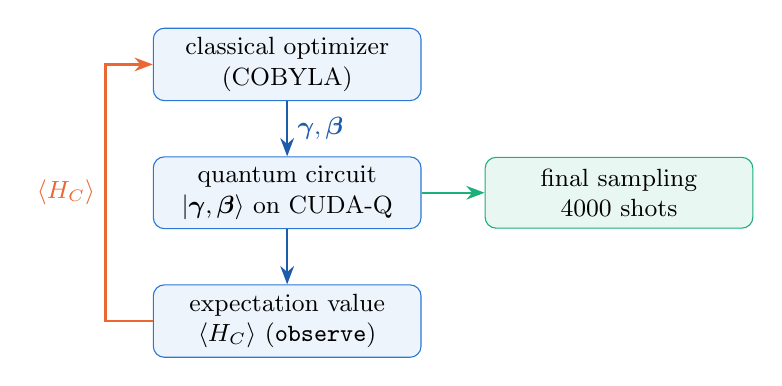
\begin{tikzpicture}[node distance=7mm, every node/.style={font=\small},
          box/.style={draw=qblue, fill=qlight, rounded corners, align=center, minimum width=34mm, minimum height=9mm}]
        \node[box] (opt) {classical optimizer\\(COBYLA)};
        \node[box, below=of opt] (qpu) {quantum circuit\\$\ket{\bg,\bb}$ on CUDA-Q};
        \node[box, below=of qpu] (obs) {expectation value\\$\langle H_C\rangle$ (\texttt{observe})};
        \draw[-{Stealth}, thick, qdark] (opt) -- node[right] {$\bg,\bb$} (qpu);
        \draw[-{Stealth}, thick, qdark] (qpu) -- (obs);
        \draw[-{Stealth}, thick, qorange] (obs.west) -- ++(-6mm,0) |- node[pos=0.25, left] {$\langle H_C\rangle$} (opt.west);
        \node[box, right=8mm of qpu, draw=qaqua, fill=qaqua!10] (smp) {final sampling\\4000 shots};
        \draw[-{Stealth}, thick, qaqua] (qpu) -- (smp);
      \end{tikzpicture}}
    \end{column}
    \begin{column}{0.44\textwidth}
      \begin{itemize}
        \item Angle vector (notebook): $\texttt{params} = [\gamma_1, \dots, \gamma_p, \beta_1, \dots, \beta_p]$ --- blocked, not
          interleaved.
        \item Depth $p$: more layers can only help with \emph{optimal} angles ($F_{p+1}^* \ge F_p^*$, set the extra
          angles to 0), but more parameters are harder to optimise.
        \item $p \to \infty$: $F_p^* \to C_{\max}$ (adiabatic limit).
        \item Each optimizer step = one full quantum simulation.
      \end{itemize}
    \end{column}
  \end{columns}
\end{frame}

\begin{frame}[fragile]{QAOA in pseudocode}
\begin{lstlisting}[language={}]
input : graph G = (V, E, w), depth p, initial angles theta0 = (gamma_1..p, beta_1..p)
H_C  <- sum over edges (w_ij / 2) Z_i Z_j                  # cost Hamiltonian
define prepare(theta):                                    # the parameterised circuit
    apply H to every qubit                                # |+>^n
    for l = 1..p:
        for (i, j, w) in E:  CNOT(i, j); RZ(gamma_l * w) on j; CNOT(i, j)
        for q in V:          RX(2 * beta_l) on q
define objective(theta):  return <prepare(theta)| H_C |prepare(theta)>
theta* <- classical_minimise(objective, theta0)            # COBYLA, 80 evaluations
samples <- measure prepare(theta*) S times                 # S = 4000
return the sampled bitstring z with the largest cut C(z), and <C> = W/2 - objective(theta*)
\end{lstlisting}
  \small The best \emph{evaluated} angles are used for sampling (the notebook keeps the history, not only the final point).
\end{frame}

% =====================================================================================
\section{Part 6: Exact analysis at small depth}
\begin{frame}{$p = 1$ on a single edge: derivation (1/2)}
  Goal: $\langle Z_0Z_1\rangle = \bra{++}U_C^\dagger U_M^\dagger\,Z_0Z_1\,U_MU_C\ket{++}$, \ $U_C = e^{-i\gamma Z_0Z_1/2}$, $U_M = e^{-i\beta(X_0+X_1)}$.
  \begin{block}{Step 1: through the mixer (each qubit separately)}
    With $c = \cos2\beta$, $s = \sin2\beta$:
    \[ U_M^\dagger Z_0Z_1U_M = (cZ_0 + sY_0)(cZ_1 + sY_1) = c^2Z_0Z_1 + cs\,(Z_0Y_1 + Y_0Z_1) + s^2Y_0Y_1 . \]
  \end{block}
  \begin{block}{Step 2: through the cost gate}
    $Z_0Z_1$ and $Y_0Y_1$ commute with $Z_0Z_1$: unchanged. $Y_0Z_1$ anticommutes, so
    \[ U_C^\dagger(Y_0Z_1)U_C = Y_0Z_1e^{-i\gamma Z_0Z_1} = \cos\gamma\,Y_0Z_1 - i\sin\gamma\,Y_0Z_0 = \cos\gamma\,Y_0Z_1 + \sin\gamma\,X_0 \]
    (using $YZ = iX$); likewise $Z_0Y_1 \to \cos\gamma\,Z_0Y_1 + \sin\gamma\,X_1$.
  \end{block}
\end{frame}

\begin{frame}{$p = 1$ on a single edge: derivation (2/2)}
  \begin{columns}[T]
    \begin{column}{0.50\textwidth}
      \begin{block}{Step 3: evaluate in $\ket{++}$}
        $\langle X_0\rangle = \langle X_1\rangle = 1$; every term with a $Y$ or a single $Z$ has expectation 0; $\langle Z_0Z_1\rangle = \langle Y_0Y_1\rangle = 0$.
        \[ \langle Z_0Z_1\rangle = 2cs\sin\gamma = \sin4\beta\,\sin\gamma \]
        \[ F_1(\gamma,\beta) = \tfrac12\big(1 - \sin4\beta\,\sin\gamma\big) \]
      \end{block}
      \begin{itemize}
        \item Maximum $F_1 = 1$ at $\sin4\beta\sin\gamma = -1$, e.g.\ $(\gamma, \beta) = (\frac\pi2, -\frac\pi8)$.
        \item At $(\frac\pi2, +\frac\pi8)$: $F_1 = 0$ --- the edge is \hl{never} cut.
      \end{itemize}
    \end{column}
    \begin{column}{0.46\textwidth}
      \centering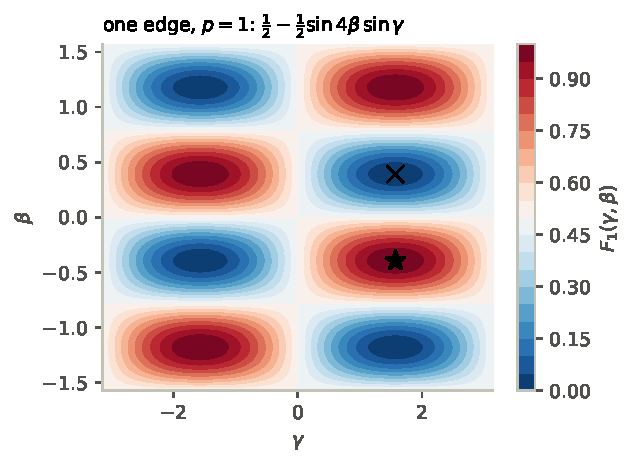
\includegraphics[width=\textwidth]{landscape_edge}\\
      \small $\star$ optimum, $\times$ worst point. CUDA-Q values agree with the formula to $10^{-9}$.
    \end{column}
  \end{columns}
\end{frame}

\begin{frame}{Sign conventions: textbook versus notebook}
  \begin{columns}[T]
    \begin{column}{0.50\textwidth}
      \begin{block}{Two common conventions}
        \small
        textbook (Farhi et al.): $e^{-i\gamma C}$\\
        notebook: $e^{-i\gamma H_C}$ with $H_C = \frac W2 - C$\\[1mm]
        $e^{-i\gamma C} = e^{-i\gamma W/2}e^{+i\gamma H_C}$: the same circuit with \hl{$\gamma \to -\gamma$}.
      \end{block}
      Single edge, textbook form: $F_1 = \tfrac12 + \tfrac12\sin4\beta\sin\gamma$ --- optimum at $(\frac\pi2, \frac\pi8)$,
      the \emph{worst} point in the notebook's convention.
    \end{column}
    \begin{column}{0.46\textwidth}
      \begin{alertblock}{Rule of thumb}
        Always translate literature angles before using them in \texttt{QAOA.ipynb}: flip the sign of every $\gamma$
        (equivalently of every $\beta$). Adding a constant to $H_C$ is harmless (global phase); a sign change is not.
      \end{alertblock}
      \begin{block}{Small-angle check}
        One edge: $\Delta F_1 \approx -2\beta\gamma$. Positive $\gamma$ and positive $\beta$ \emph{lower} the cut.
      \end{block}
    \end{column}
  \end{columns}
\end{frame}

\begin{frame}{$p = 1$ for triangle-free graphs}
  The same Heisenberg calculation for an edge $(u, v)$ whose end nodes have degrees $d_u, d_v$ and no common neighbour gives
  (notebook convention; Wang, Hadfield, Jiang, Rieffel 2018 in the textbook convention):
  \begin{block}{Edge correlator}
    \[ \langle Z_uZ_v\rangle = \tfrac12\,\sin4\beta\,\sin\gamma\,\big(\cos^{d_u-1}\gamma + \cos^{d_v-1}\gamma\big), \qquad
       \langle C_{uv}\rangle = \tfrac12\big(1 - \langle Z_uZ_v\rangle\big) \]
  \end{block}
  \begin{columns}[T]
    \begin{column}{0.48\textwidth}
      \begin{exampleblock}{Ring $C_n$ ($d = 2$)}
        $\langle C_{uv}\rangle = \tfrac12 - \tfrac14\sin4\beta\sin2\gamma \le \tfrac34$ at $(\frac\pi4, -\frac\pi8)$.\\
        Even ring: $r = 3/4$ (numerical optimum: \numringone).
      \end{exampleblock}
    \end{column}
    \begin{column}{0.48\textwidth}
      \begin{exampleblock}{Single edge ($d = 1$)}
        $\cos^0\gamma = 1$: recovers $\sin4\beta\sin\gamma$.\\
        \textbf{3-regular graphs:} $r \ge 0.6924$ at $p = 1$ (Farhi et al.\ 2014).
      \end{exampleblock}
    \end{column}
  \end{columns}
\end{frame}

\begin{frame}{The $p = 1$ landscape of the notebook's graph}
  \begin{columns}[c]
    \begin{column}{0.5\textwidth}
      \centering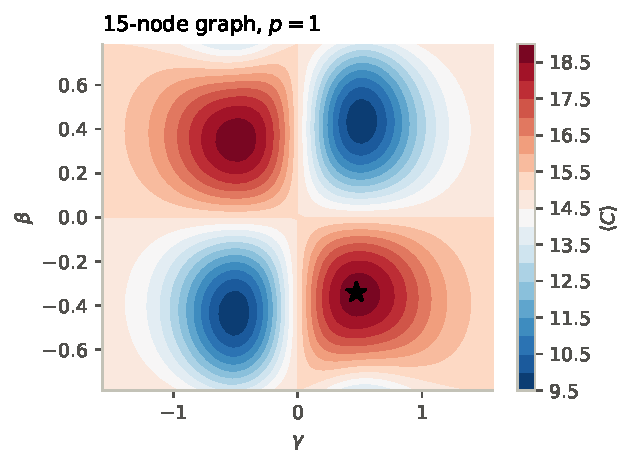
\includegraphics[width=\textwidth]{landscape_repo}
    \end{column}
    \begin{column}{0.46\textwidth}
      \begin{itemize}
        \item $\langle C\rangle$ on a $61\times61$ grid of $(\gamma, \beta)$ (NumPy; the best point re-checked with CUDA-Q).
        \item Best grid point: $\langle C\rangle = \numponebest$ at $(\gamma, \beta) \approx (\numponegamma, \numponebeta)$ ---
          again $\gamma$ and $\beta$ of \hl{opposite signs}.
        \item The point symmetry $(\gamma, \beta) \to (-\gamma, -\beta)$ is visible; blue regions are \emph{worse} than random.
        \item $p = 2$ adds two more angles and reaches $20.53$ (Part 9).
      \end{itemize}
    \end{column}
  \end{columns}
\end{frame}

\begin{frame}{Depth, light cones and the ring}
  \begin{columns}[c]
    \begin{column}{0.48\textwidth}
      \begin{block}{Light cone}
        In $U^\dagger Z_uZ_vU$ every cost layer adds the neighbours of the current support; gates further away cancel.
        After $p$ layers $\langle Z_uZ_v\rangle$ depends only on the nodes within distance $p$ of the edge --- on a ring,
        $2p + 2$ qubits.
      \end{block}
      \begin{itemize}
        \item Fixed-$p$ QAOA is a \key{local} algorithm.
        \item Rings with $n \ge 2p + 2$: every edge sees the same path, so $r$ does not depend on $n$.
        \item Ring, optimised numerically: $p = 1, 2, 3$: \numringone, \numringtwo, \numringthree{} $=$ $\frac34, \frac56, \frac78$.
      \end{itemize}
    \end{column}
    \begin{column}{0.48\textwidth}
      \centering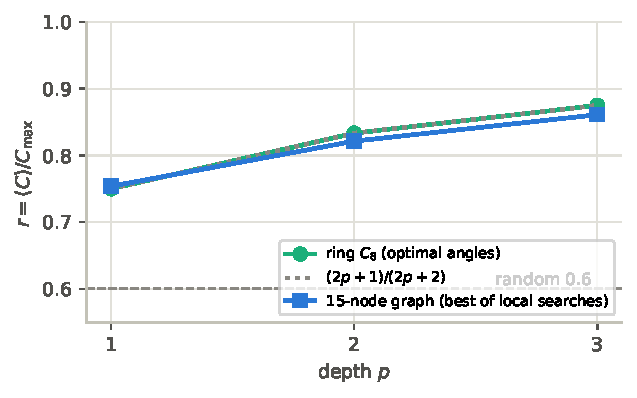
\includegraphics[width=\textwidth]{ratio_vs_depth}\\
      \small 15-node graph: best values found by local optimisation from several starts (not proven global):
      $p = 1, 2, 3$: \numrepoone, \numrepotwo, \numrepothree.
    \end{column}
  \end{columns}
\end{frame}

\begin{frame}{Exactly solvable at $p = 1$: the triangle}
  \begin{columns}[T]
    \begin{column}{0.52\textwidth}
      \begin{itemize}
        \item $H_C$ on $K_3$ has only two eigenvalues: $+\frac32$ on $\{000, 111\}$, $-\frac12$ on the 6 optimal strings.
        \item So $e^{-i\gamma H_C}$ only sets one relative phase $e^{-2i\gamma}$ between ``bad'' and ``good'' strings.
        \item One mixer can then remove the bad amplitudes completely.
      \end{itemize}
      \begin{exampleblock}{Result (checked with CUDA-Q)}
        At $\gamma^* = \arctan\frac{1}{\sqrt2} \approx 0.6155$, $\beta^* = -\gamma^*/2$: $F_1 = 2 = C_{\max}$, i.e.\ $r = 1$ and
        $P_{\text{opt}} = 1$.
      \end{exampleblock}
    \end{column}
    \begin{column}{0.44\textwidth}
      \begin{alertblock}{Do not generalise}
        Exact solution at $p = 1$ is special to tiny, highly symmetric graphs (one edge, the triangle). The ring already
        stops at $\frac34$, and general graphs need larger $p$ --- with no fixed guarantee.
      \end{alertblock}
    \end{column}
  \end{columns}
\end{frame}

% =====================================================================================
\section{Part 7: Worked examples}
\begin{frame}{Worked example 1: one edge, traced amplitude by amplitude}
  \small
  $\gamma = \frac\pi2$, $\beta = \frac\pi8$, order $\ket{00}, \ket{01}, \ket{10}, \ket{11}$ (notebook convention).
  \begin{center}
  \begin{tabular}{lcccc}
    \toprule after & $\ket{00}$ & $\ket{01}$ & $\ket{10}$ & $\ket{11}$\\ \midrule
    $H\otimes H$ & $\frac12$ & $\frac12$ & $\frac12$ & $\frac12$\\
    CNOT, $R_Z(\frac\pi2)$ on $q_1$, CNOT & $\frac12e^{-i\pi/4}$ & $\frac12e^{+i\pi/4}$ & $\frac12e^{+i\pi/4}$ & $\frac12e^{-i\pi/4}$\\
    probabilities so far & $\frac14$ & $\frac14$ & $\frac14$ & $\frac14$\\
    $R_X(\frac\pi4)\otimes R_X(\frac\pi4)$: probabilities & $0.5$ & $0$ & $0$ & $0.5$\\ \bottomrule
  \end{tabular}
  \end{center}
  \begin{itemize}
    \item The cost layer gives cut strings the relative phase $\gamma = 90^\circ$; probabilities are unchanged.
    \item The mixer turns the phases into probabilities: here \hl{all} weight goes to the \emph{uncut} strings, because
      $\sin4\beta\sin\gamma = +1$ (formula: $P(\text{cut}) = \frac12(1 - \sin4\beta\sin\gamma) = 0$).
    \item With $\beta = -\frac\pi8$ the same circuit returns $01$ or $10$ with certainty.
  \end{itemize}
\end{frame}

\begin{frame}{Worked example 2: the path $0 - 1 - 2$ at $p = 1$}
  \begin{columns}[T]
    \begin{column}{0.52\textwidth}
      $(\gamma, \beta) = (\frac\pi2, -\frac\pi8)$: $\sin\gamma = 1$, $\cos\gamma = 0$, $\sin4\beta = -1$.
      \begin{enumerate}
        \item Edge $(0,1)$: $d_0 = 1$, $d_1 = 2$:\\ $\langle Z_0Z_1\rangle = \frac12(-1)(1)(\cos^0\gamma + \cos^1\gamma) = \frac12(-1)(1 + 0) = -\frac12$.
        \item Edge $(1,2)$: the same by symmetry.
        \item $\langle C\rangle = 2\cdot\frac12\big(1 + \frac12\big) = 1.5$, \ $r = 1.5/2 = 0.75$.
      \end{enumerate}
    \end{column}
    \begin{column}{0.44\textwidth}
      \begin{exampleblock}{State-vector check}
        $P(010) = P(101) = 0.3125$; each other string $0.0625$.\\
        $P_{\text{opt}} = 0.625$.\\
        $\langle C\rangle = 2(0.625) + 1(4\times0.0625) = 1.5$ \checkmark
      \end{exampleblock}
      \small A sampler finds the optimum with probability $0.625$ per shot although the average ratio is only $0.75$.
    \end{column}
  \end{columns}
\end{frame}

\begin{frame}{Worked example 3: counting the default circuit}
  \begin{columns}[T]
    \begin{column}{0.5\textwidth}
      $n = 15$, $|E| = 30$, $p = 2$:
      \begin{center}\small
      \begin{tabular}{lr}
        \toprule gate & count\\ \midrule
        $H$ (initial state) & $n = 15$\\
        CNOT (cost) & $2p|E| = 120$\\
        $R_Z$ (cost) & $p|E| = 60$\\
        $R_X$ (mixer) & $pn = 30$\\ \midrule
        total (no measurements) & $225$\\
        parameters & $2p = 4$\\ \bottomrule
      \end{tabular}
      \end{center}
    \end{column}
    \begin{column}{0.46\textwidth}
      These agree with the statistics recorded by the notebook: \texttt{h 15, cx 120, rz 60, rx 30, mz 15}, depth 64.
      \begin{block}{Scaling}
        Two-qubit gates grow like $2p|E|$; for $G(n, 0.3)$, $|E| \approx 0.15\,n^2$. At $n = 25$, $|E| = 90$:
        $615$ gates, $360$ CNOTs per circuit ($p = 2$).
      \end{block}
    \end{column}
  \end{columns}
\end{frame}

% =====================================================================================
\section{Part 8: CUDA-Q implementation}
\begin{frame}{The structure of \texttt{QAOA.ipynb}}
  \begin{columns}[T]
    \begin{column}{0.5\textwidth}
      \footnotesize
      \begin{enumerate}\itemsep0pt
        \item Problem statement and mathematics
        \item Imports and version check
        \item \key{Input parameters} (the only cell to edit)
        \item Example inputs: build the graph, brute-force reference
        \item Benchmark utilities, backend selection
        \item Expected output: memory, time estimate
        \item Circuit generation, drawing, statistics, QIR export
        \item \key{Execution}: optimisation + sampling, live memory monitor
        \item Results and plots
        \item Final benchmark report (JSON + PNG in \texttt{exports/qaoa/})
      \end{enumerate}
    \end{column}
    \begin{column}{0.46\textwidth}
      \begin{block}{Section 3 defaults}
        \small
        \texttt{N\_QUBITS = 15}, \texttt{GRAPH = "example"}, \texttt{EDGE\_PROBABILITY = 0.3}\\
        \texttt{QAOA\_LAYERS = 2}, \texttt{OPTIMIZER = "COBYLA"}\\
        \texttt{MAX\_EVALUATIONS = 80}, \texttt{INITIAL\_PARAMETERS = "ramp"}\\
        \texttt{OBJECTIVE\_SHOTS = None} (exact), \texttt{SHOTS = 4000}, \texttt{SEED = 42}\\
        \texttt{BRUTE\_FORCE\_MAX\_NODES = 22}, \texttt{BACKEND = "auto"}
      \end{block}
      \small Graphs: \texttt{"example"} (random), \texttt{"ring"}, \texttt{"complete"}, \texttt{"custom"} (weighted edge list).
    \end{column}
  \end{columns}
\end{frame}

\begin{frame}[fragile]{Building the instance and the classical reference (Section 4)}
\begin{lstlisting}[basicstyle=\ttfamily\fontsize{6.4}{7.6}\selectfont]
graph_rng = np.random.default_rng(SEED)                      # reproducible random graph
edges = [(i, j, 1.0) for i in range(N_QUBITS) for j in range(i + 1, N_QUBITS)
         if graph_rng.random() < EDGE_PROBABILITY]           # each pair with probability 0.3
edge_i = [e[0] for e in edges]; edge_j = [e[1] for e in edges]; edge_w = [e[2] for e in edges]
total_weight = float(sum(edge_w))                            # W: a random split has <C> = W/2

def brute_force_maxcut():                                    # all 2^N splits, vectorised
    index = np.arange(2 ** N_QUBITS, dtype=np.int64)
    values = np.zeros(2 ** N_QUBITS)
    for i, j, w in edges:                                    # bit i of z XOR bit j of z
        values += w * (((index >> (N_QUBITS - 1 - i)) ^ (index >> (N_QUBITS - 1 - j))) & 1)
    best = values.max()
    optimal = [format(int(z), f"0{N_QUBITS}b") for z in np.flatnonzero(np.isclose(values, best))]
    return best, optimal
\end{lstlisting}
  \small Node 0 is the most significant bit and is written first. Output of the default: 30 edges, $W = 30$, max cut 25,
  4 optimal splits, $0.01$ s. For $N > 22$ a greedy local search replaces brute force.
\end{frame}

\begin{frame}[fragile]{The cost Hamiltonian and the initial angles (Section 7a)}
\begin{lstlisting}[basicstyle=\ttfamily\fontsize{6.4}{7.6}\selectfont]
def cost_hamiltonian():
    """H_C = sum_(i,j) w_ij/2 Z_i Z_j  (maximising the cut <=> minimising <H_C>)."""
    hamiltonian = None
    for i, j, w in edges:
        term = 0.5 * w * cudaq.spin.z(i) * cudaq.spin.z(j)   # one Z_i Z_j term per edge
        hamiltonian = term if hamiltonian is None else hamiltonian + term
    return hamiltonian

if INITIAL_PARAMETERS == "ramp":
    initial_params = np.concatenate([np.linspace(0.2, 0.6, QAOA_LAYERS),   # gamma_1..gamma_p rising
                                     np.linspace(0.6, 0.2, QAOA_LAYERS)])  # beta_1..beta_p falling
\end{lstlisting}
  \begin{itemize}\small
    \item \texttt{cudaq.spin.z(i)} is the operator $Z_i$; products and sums build a \texttt{SpinOperator} with 30 terms.
    \item No constant: $\langle C\rangle$ is recovered as \texttt{total\_weight / 2 - energy}.
    \item $p = 2$ ramp: $\bg = (0.2, 0.6)$, $\bb = (0.6, 0.2)$ --- both positive (see the results part).
  \end{itemize}
\end{frame}

\begin{frame}[fragile]{The QAOA kernel, line by line (Section 7a)}
  \begin{columns}[T]
    \begin{column}{0.58\textwidth}
\begin{lstlisting}
@cudaq.kernel
def qaoa_state(n: int, edge_i: list[int],
               edge_j: list[int], weights: list[float],
               layers: int, params: list[float]):
    qubits = cudaq.qvector(n)          # |0...0>
    h(qubits)                          # |+>^n
    for layer in range(layers):
        gamma = params[layer]
        beta = params[layers + layer]
        for e in range(len(edge_i)):   # cost layer
            x.ctrl(qubits[edge_i[e]], qubits[edge_j[e]])
            rz(gamma * weights[e], qubits[edge_j[e]])
            x.ctrl(qubits[edge_i[e]], qubits[edge_j[e]])
        for q in range(n):             # mixer layer
            rx(2.0 * beta, qubits[q])
\end{lstlisting}
    \end{column}
    \begin{column}{0.40\textwidth}
      \small
      \begin{itemize}
        \item \texttt{@cudaq.kernel}: compiled to MLIR/QIR, then JIT-compiled (``compilation time'' in the report).
        \item \texttt{h(qubits)} broadcasts $H$ over the register.
        \item \texttt{params[layer]}, \texttt{params[layers+layer]}: the blocked layout $[\bg, \bb]$.
        \item \texttt{x.ctrl(c, t)} is a CNOT; with \texttt{rz(gamma*w)}: $e^{-i\gamma\frac w2Z_iZ_j}$.
        \item \texttt{rx(2*beta)} $= e^{-i\beta X}$.
        \item \texttt{qaoa\_sample} is the same body followed by \texttt{mz(qubits)}.
      \end{itemize}
    \end{column}
  \end{columns}
\end{frame}

\begin{frame}[fragile]{Objective, optimizer and sampling (Section 8)}
\begin{lstlisting}
def objective(params):
    result = cudaq.observe(kernels["state"], H_C, N_QUBITS, edge_i, edge_j, edge_w,
                           QAOA_LAYERS, list(params), **observe_kwargs)   # exact, or shots
    energy = result.expectation()                    # <H_C>
    history_cut.append(total_weight / 2 - energy)    # record <C>
    history_params.append(np.array(params, dtype=float))
    return energy                                     # SciPy MINIMISES <H_C>

opt = minimize(objective, initial_params, method="COBYLA",
               options={"maxiter": MAX_EVALUATIONS, "rhobeg": 0.2})
best_params = history_params[int(np.argmax(history_cut))]   # best evaluated angles
counts = cudaq.sample(kernels["sample"], N_QUBITS, edge_i, edge_j, edge_w,
                      QAOA_LAYERS, best_params.tolist(), shots_count=SHOTS)
\end{lstlisting}
  \small \texttt{observe} returns the exact $\langle H_C\rangle$ on simulators (or a shot estimate if \texttt{OBJECTIVE\_SHOTS} is set; always
  on hardware). COBYLA is derivative-free; \texttt{rhobeg} is its initial trust-region radius. Other choices:
  Nelder-Mead, Powell, L-BFGS-B (finite differences, $2p+1$ runs per gradient).
\end{frame}

\begin{frame}[fragile]{Result extraction (Sections 8--9)}
\begin{lstlisting}
samples = sorted(((b, c, cut_value(b)) for b, c in counts.items()),
                 key=lambda t: (-t[1], -t[2]))               # by frequency, then by cut
best_sample = max(samples, key=lambda t: (t[2], t[1]))        # largest cut seen
optimal_hits = sum(c for b, c, v in samples if np.isclose(v, max_cut))
ratio = expected_cut / max_cut                                # r = <C> / C_max
\end{lstlisting}
  \begin{columns}[T]
    \begin{column}{0.5\textwidth}
      \small
      \begin{itemize}
        \item Each key of \texttt{counts} is a bitstring (qubit/node 0 first) with its number of shots.
        \item The cut of every sample is computed \emph{classically} with \texttt{cut\_value} --- checking a candidate is cheap.
        \item Reported: best expected cut, $r$, best sampled split, $P(\text{optimal split})$, timing and memory.
      \end{itemize}
    \end{column}
    \begin{column}{0.46\textwidth}
      \begin{block}{Plots produced}
        \small Objective convergence; best split drawn on the graph; most frequent bitstrings; distribution of
        cut values; memory timeline; final report figure.
      \end{block}
    \end{column}
  \end{columns}
\end{frame}

\begin{frame}{Backends: CPU, GPU, multi-GPU, hardware}
  \footnotesize
  \begin{center}
  \resizebox{\textwidth}{!}{%
  \begin{tabular}{llll}
    \toprule \texttt{BACKEND} + \texttt{SIMULATION\_METHOD} & CUDA-Q target & memory & validated here?\\ \midrule
    \texttt{cpu} + \texttt{statevector} & \texttt{qpp-cpu} & $16\times2^n$ B & \textbf{yes} (recorded + re-run)\\
    \texttt{cpu} + \texttt{density\_matrix} & \texttt{density-matrix-cpu} & $16\times4^n$ B & no\\
    \texttt{gpu} + \texttt{statevector} & \texttt{nvidia} (fp32/fp64) & $8$ / $16\times2^n$ B & no (no GPU)\\
    \texttt{gpu} + \texttt{mps} / \texttt{tensornet} & \texttt{tensornet-mps} / \texttt{tensornet} & depends on entanglement & no (no GPU)\\
    \texttt{multi-gpu} + \texttt{statevector} & \texttt{nvidia}, option \texttt{mgpu} (MPI) & split over GPUs & no\\
    \texttt{hardware} & \texttt{quantinuum}, \texttt{ionq}, \dots & --- & no\\ \bottomrule
  \end{tabular}}
  \end{center}
  \begin{itemize}
    \item \texttt{"auto"} picks a GPU if CUDA-Q sees one, else the CPU. Unsupported pairs stop with an explanation
      (e.g.\ \texttt{cpu} + \texttt{mps}: ``needs an NVIDIA GPU'').
    \item Multi-GPU pooling needs one MPI rank per GPU: \texttt{jupyter nbconvert --to script}, then \texttt{mpiexec -np 4}.
    \item Hardware targets return samples only: the objective is then always estimated from \texttt{SHOTS} shots.
      \texttt{HARDWARE\_EMULATE = True} runs the provider's flow locally.
  \end{itemize}
\end{frame}

\begin{frame}{Memory, time estimates and exports}
  \begin{columns}[T]
    \begin{column}{0.52\textwidth}
      \centering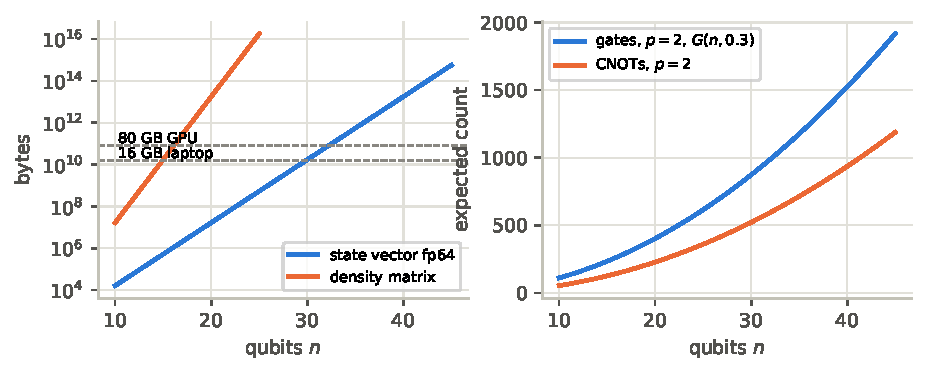
\includegraphics[width=\textwidth]{scaling}
    \end{column}
    \begin{column}{0.44\textwidth}
      \small
      \begin{itemize}
        \item Section 6 computes the state memory exactly and refuses runs above \texttt{MEMORY\_SAFETY\_FRACTION} ($80\,\%$).
        \item Time estimate: (evaluations) $\times$ (gates) $\times$ (measured time per gate), scaled by $2^n$ --- rough, about $\pm3\times$.
        \item Recorded: estimate $\sim 39.8$ s, measured $40.8$ s.
        \item Exports in \texttt{exports/qaoa/}: circuit drawing (\texttt{.txt}, \texttt{.png}), full circuit as QIR
          (\texttt{.ll}), report (\texttt{.json}, \texttt{.png}).
      \end{itemize}
    \end{column}
  \end{columns}
\end{frame}

% =====================================================================================
\section{Part 9: Results}
\begin{frame}{The default instance}
  \centering
  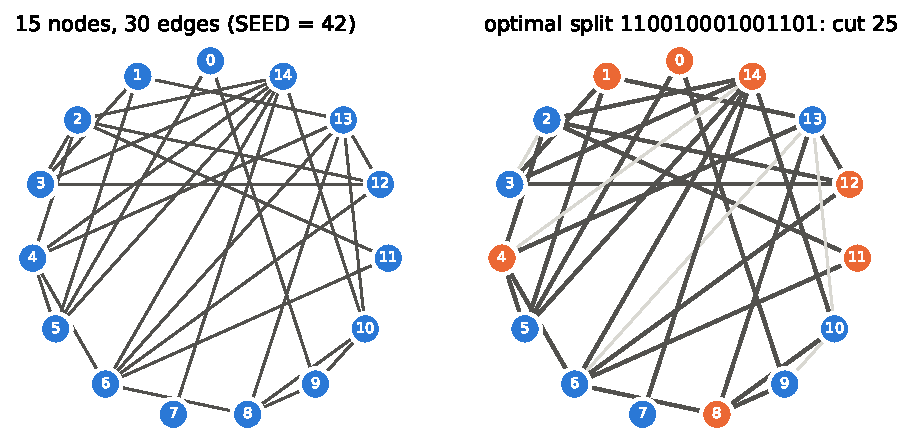
\includegraphics[width=0.78\textwidth]{graph15}\\
  \raggedright\small
  $15$ nodes, \numnedges{} unit edges, $W/2 = 15$. Exact optimum (brute force over $32\,768$ splits): $C_{\max} = \numcmax$;
  \numnopt{} optimal bitstrings $=$ 2 partitions (complementary pairs). Node 10 can join either side in one of them.
\end{frame}

\begin{frame}{Recorded versus re-executed results}
  \footnotesize
  \begin{center}
  \resizebox{0.92\textwidth}{!}{%
  \begin{tabular}{lcc}
    \toprule & \textbf{previously recorded} (notebook outputs) & \textbf{re-executed for this lecture}\\ \midrule
    machine & 4 vCPU Xeon, 16.9 GB & laptop, WSL Ubuntu, 12 threads, 3.9 GB\\
    CUDA-Q / target & 0.16.0 / \texttt{qpp-cpu} & 0.16.0 / \texttt{qpp-cpu}\\
    COBYLA evaluations & 80 (budget reached) & 75 (trust region at lower bound)\\
    best $\langle C\rangle$, $r$ & 20.5336, 0.8213 & 20.5336, 0.8213\\
    best sampled cut & 25 (\texttt{110010001001101}) & 25 (\texttt{110010001001101})\\
    $P(\text{optimal split})$ & 0.0600 (240 / 4000) & 0.0600 (240 / 4000)\\
    execution cell & 40.8 s & 183.9 s\\ \bottomrule
  \end{tabular}}
  \end{center}
  \begin{itemize}
    \item Same seed, same versions: the optimisation results agree to all printed digits; the number of optimizer steps
      differs slightly (floating-point summation order with different thread counts).
    \item Timings are machine-specific. GPU, multi-GPU and hardware paths were \hl{not} executed (no GPU available).
    \item The lecture's own script (\texttt{make\_figures.py}) obtains $\langle C\rangle = \numbestcut$, $r = \numratio$ after
      \numnevals{} evaluations; CUDA-Q and NumPy states agree with fidelity \numfid.
  \end{itemize}
\end{frame}

\begin{frame}{Convergence of the optimizer}
  \centering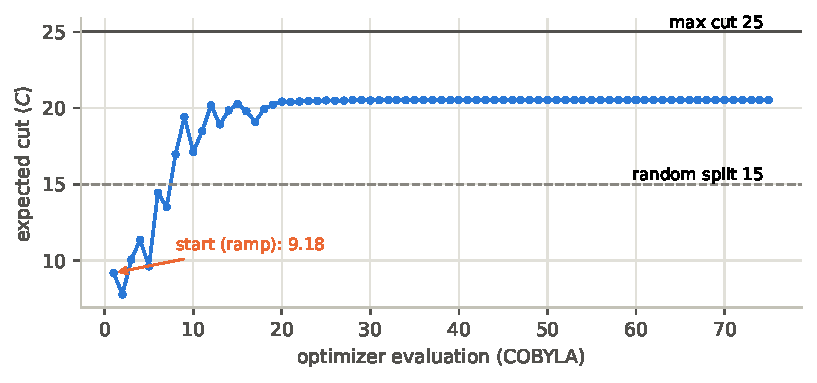
\includegraphics[width=0.66\textwidth]{convergence}\\
  \raggedright\footnotesize
  \begin{itemize}
    \item The \hl{ramp start gives $\langle C\rangle = \numstart$ --- below random guessing ($15$)}. Reason: $\gamma, \beta > 0$ in the
      notebook's convention heads towards \emph{small} cuts (Part 6). COBYLA leaves this region within a few steps.
    \item Best angles found: $\bg = (\numgammaa, \numgammab)$, $\bb = (\numbetaa, \numbetab)$. Because $F_p$ has period
      $\pi/2$ in each $\beta_l$, $\beta_1 = \numbetaa \equiv \numbetaa - \pi/2 = -0.454$: the optimizer ended with $\gamma > 0$ and
      $\beta < 0$ --- \hl{opposite signs}, as the analysis predicts.
  \end{itemize}
\end{frame}

\begin{frame}{What the optimised circuit produces}
  \begin{columns}[c]
    \begin{column}{0.56\textwidth}
      \centering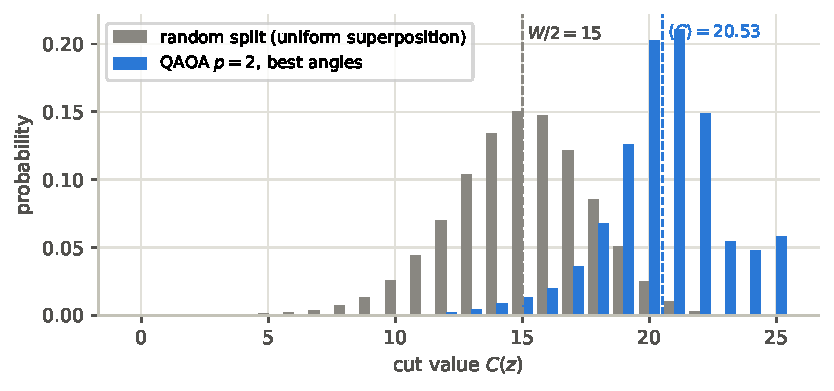
\includegraphics[width=0.92\textwidth]{cut_distribution}\\[1mm]
      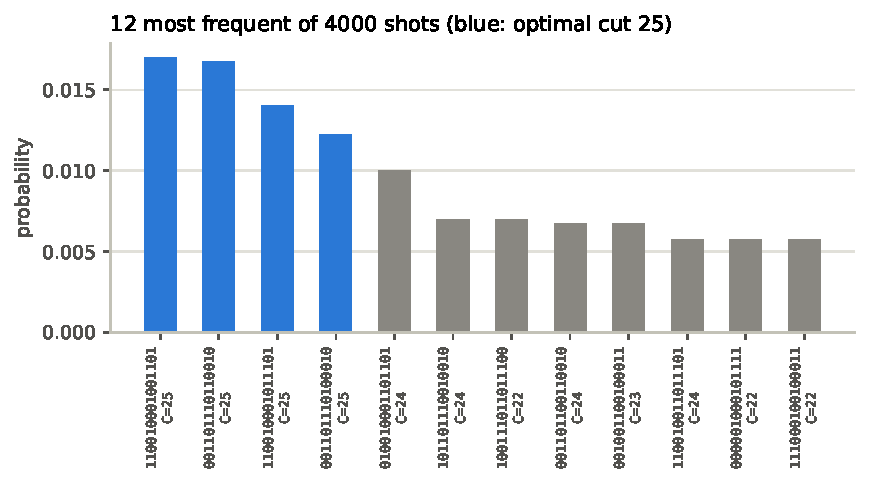
\includegraphics[width=0.92\textwidth]{top_bitstrings}
    \end{column}
    \begin{column}{0.42\textwidth}
      \footnotesize
      \begin{itemize}
        \item The distribution of cut values moves from the random bell curve (mean 15, $\sigma = 2.74$) to mean $20.53$.
        \item $P(C = 25)$: $\numprandopt$ (random) $\to$ $\numpqaoaopt$ (QAOA, exact from the state vector; the 4000-shot
          estimate is $0.0600$): about $475\times$ more likely.
        \item The 4 most frequent strings are exactly the 4 optimal ones; complementary strings have nearly equal counts
          ($68/67$, $56/49$) --- the $z \leftrightarrow \bar z$ symmetry, up to shot noise.
        \item Mean cut over 4000 shots: \numshotmean{} (exact $\langle C\rangle = 20.53$).
      \end{itemize}
    \end{column}
  \end{columns}
\end{frame}

\begin{frame}{Interpreting the numbers correctly}
  \begin{columns}[T]
    \begin{column}{0.5\textwidth}
      \begin{block}{Approximation ratio $r = 0.82$}
        An \emph{average} over the output distribution. It does \emph{not} mean $82\,\%$ of shots are optimal ($6\,\%$ are).
      \end{block}
      \begin{block}{Improvement over random}
        Random guessing already has $r = 15/25 = 0.6$. A stricter measure:
        \[ \eta = \frac{\langle C\rangle - W/2}{C_{\max} - W/2} = \frac{20.53 - 15}{10} = \numeta . \]
      \end{block}
    \end{column}
    \begin{column}{0.46\textwidth}
      \begin{block}{QAOA as a sampler}
        With $P_{\text{opt}} = 0.06$, $75$ shots already give $99\,\%$ probability of seeing an optimum
        ($1 - 0.94^{75} \ge 0.99$). The best of 4000 shots was optimal.
      \end{block}
      \begin{alertblock}{No speed-up claim}
        This 15-node instance is brute-forced classically in $0.01$ s. The value of the experiment is a reproducible
        benchmark of the method and of the simulator.
      \end{alertblock}
    \end{column}
  \end{columns}
\end{frame}

\begin{frame}{Performance analysis of the recorded run}
  \begin{columns}[T]
    \begin{column}{0.5\textwidth}
      \small
      \begin{center}
      \begin{tabular}{lr}
        \toprule phase (recorded) & time\\ \midrule
        circuit construction & 0.019 s\\
        compilation (MLIR + JIT) & 0.045 s\\
        quantum execution (80 \texttt{observe}) & 40.01 s\\
        final sampling (4000 shots) & 0.60 s\\
        optimizer + Python overhead & 0.13 s\\ \midrule
        execution cell & 40.84 s\\ \bottomrule
      \end{tabular}
      \end{center}
    \end{column}
    \begin{column}{0.46\textwidth}
      \small
      \begin{itemize}
        \item $40.01/80 \approx 0.50$ s per evaluation, $\approx 2.2$ ms per gate --- the calibration predicted $2.18$ ms.
        \item Simulation dominates completely; the classical optimizer costs almost nothing.
        \item Peak host RAM 0.89 GB; the state itself is only $0.5$ MB --- the Python/CUDA-Q runtime dominates memory at this size.
        \item Model: $n = 25$, $|E| = 90$ would take $\approx 2.8\times10^3\times$ longer on the same CPU ($\approx$ 31 h): use a GPU.
      \end{itemize}
    \end{column}
  \end{columns}
\end{frame}

% =====================================================================================
\section{Part 10: Limits and outlook}
\begin{frame}{Limitations and challenges}
  \small
  \begin{columns}[T]
    \begin{column}{0.5\textwidth}
      \begin{itemize}
        \item \key{Optimisation landscape}: many local optima; results depend on the start point (see the ramp).
        \item \key{Gradients}: exact parameter-shift gradients need 2 runs \emph{per gate} using the angle ---
          $2p(|E| + n) = 180$ runs for the default, versus $5$ for finite differences.
        \item \key{Shot noise}: on hardware each objective value has error $\sigma_C/\sqrt S$ ($\approx 0.08$ for $\sigma_C = 2.5$, $S = 1000$).
        \item \key{Locality}: fixed $p$ sees only $p$-neighbourhoods; low-depth QAOA provably cannot reach the optimum on some graph families (Bravyi et al.\ 2020).
      \end{itemize}
    \end{column}
    \begin{column}{0.46\textwidth}
      \begin{itemize}
        \item \key{Guarantees}: $p = 1$ gives $0.6924$ on 3-regular graphs; Goemans--Williamson gives $0.878$ classically.
        \item \key{Classical simulation}: $16\times2^n$ bytes --- 32 qubits fit on one 80 GB GPU (fp64), 36 qubits need 16 such GPUs.
        \item \key{No demonstrated quantum advantage} for Max-Cut so far.
      \end{itemize}
    \end{column}
  \end{columns}
\end{frame}

\begin{frame}{Noise and hardware considerations}
  \begin{columns}[T]
    \begin{column}{0.5\textwidth}
      \footnotesize
      \begin{itemize}
        \item Each CNOT has an error rate $\varepsilon$ (typically $10^{-3}$--$10^{-2}$ today).
        \item Illustrative global-depolarising model: with probability $F = (1-\varepsilon)^{N_{\text{CNOT}}}$ the ideal output,
          otherwise a random bitstring:
          \[ \langle C\rangle_{\text{noisy}} = F\langle C\rangle_{\text{ideal}} + (1 - F)\,\tfrac W2 . \]
        \item Default ($120$ CNOTs, $\varepsilon = 0.5\,\%$): $F = 0.55$, $\langle C\rangle \approx 18.0$.
        \item \key{Connectivity}: on hardware with nearest-neighbour coupling, distant edges need SWAP gates (3 CNOTs each).
        \item Deeper circuits help in theory but cost fidelity: an optimal $p$ exists for given hardware.
      \end{itemize}
    \end{column}
    \begin{column}{0.46\textwidth}
      \centering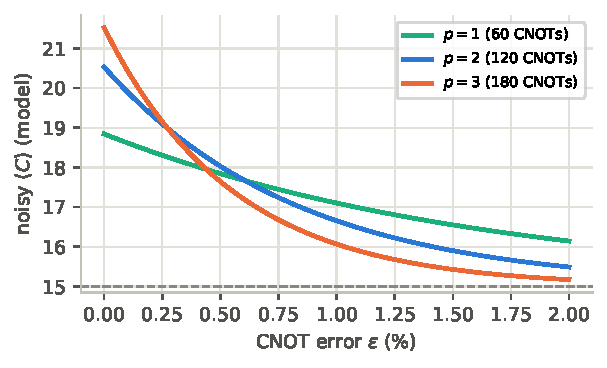
\includegraphics[width=\textwidth]{noise_model}\\
      \small The model is an assumption for illustration, not a hardware measurement. \texttt{Noise\_Simulation.ipynb}
      shows real CUDA-Q noise channels.
    \end{column}
  \end{columns}
\end{frame}

\begin{frame}{Advanced QAOA and current research}
  \footnotesize
  \begin{columns}[T]
    \begin{column}{0.5\textwidth}
      \begin{block}{Better angles}
        \begin{itemize}
          \item \key{INTERP} (Zhou et al.\ 2020): interpolate optimised depth-$p$ angles to start depth $p+1$; e.g.\ $(0.4, 0.8) \to (0.4, 0.6, 0.8)$.
          \item \key{Parameter transfer / concentration}: optimal angles depend mainly on local graph structure, so angles from small graphs work on large ones.
        \end{itemize}
      \end{block}
      \begin{block}{Better ansatz}
        \begin{itemize}
          \item \key{Warm-start QAOA}: initial state from a classical relaxation.
          \item \key{ADAPT-QAOA}: grow mixers from an operator pool by gradient.
        \end{itemize}
      \end{block}
    \end{column}
    \begin{column}{0.46\textwidth}
      \begin{block}{Other problems}
        \begin{itemize}
          \item \key{Quantum Alternating Operator Ansatz} (Hadfield et al.\ 2019): mixers such as the XY mixer that keep constrained
            problems (graph colouring, TSP) in the feasible subspace.
          \item \key{Recursive QAOA} (Bravyi et al.\ 2020): fix variables from strong correlations $\langle Z_iZ_j\rangle$ and recurse.
        \end{itemize}
      \end{block}
      \small None of these variants is implemented in \texttt{QAOA.ipynb}; they are natural extensions of its code.
    \end{column}
  \end{columns}
\end{frame}

\begin{frame}{Try it yourself: \texttt{QAOA.ipynb}}
  \begin{columns}[T]
    \begin{column}{0.5\textwidth}
      \begin{enumerate}
        \item Install: \texttt{pip install -r requirements.txt}
        \item Open \texttt{QAOA.ipynb} and run all cells.
        \item Change only Section 3:
          \begin{itemize}
            \item \texttt{GRAPH = "ring"}, \texttt{N\_QUBITS = 8}: compare $r$ with $\frac34$, $\frac56$, \dots
            \item \texttt{INITIAL\_PARAMETERS = [0.2, 0.6, -0.6, -0.2]}: start with opposite signs
            \item \texttt{QAOA\_LAYERS = 3}, \texttt{MAX\_EVALUATIONS = 200}
          \end{itemize}
      \end{enumerate}
    \end{column}
    \begin{column}{0.46\textwidth}
      \begin{block}{Experiments}
        \begin{itemize}
          \item \texttt{OBJECTIVE\_SHOTS = 1000}: optimise with shot noise, as on hardware
          \item \texttt{OPTIMIZER = "L-BFGS-B"}: gradient-based (finite differences)
          \item \texttt{N\_QUBITS = 24}, \texttt{BACKEND = "gpu"}: compare execution times
          \item \texttt{GRAPH = "custom"} with weights, including negative ones
        \end{itemize}
      \end{block}
      \small The notebook checks every result against the brute-force optimum and reports time and memory.
    \end{column}
  \end{columns}
\end{frame}

% =====================================================================================
\section{Part 11: Practice and summary}
\begin{frame}{Exercises}
  \begin{enumerate}
    \item Write the cut of the square $0{-}1{-}2{-}3{-}0$ as a QUBO polynomial and as $\frac W2 - H_C$.
    \item How many bitstrings and how many partitions does a 20-node graph have?
    \item Show that CNOT$\,(I\otimes R_Z(\theta))\,$CNOT acts on $\ket{11}$ as $e^{-i\theta/2}$.
    \item For one edge and $p = 1$, find all $(\gamma, \beta) \in [0, \pi]\times[-\frac\pi4, \frac\pi4]$ with $F_1 = 1$.
    \item A ring $C_{10}$ at $p = 1$ with optimal angles: what is the expected cut?
    \item Gates and CNOTs of the notebook's circuit for $n = 12$, $|E| = 20$, $p = 3$?
    \item Convert the textbook optimum $(\gamma, \beta) = (\frac\pi4, \frac\pi8)$ for a ring into the notebook's convention.
    \item With $P_{\text{opt}} = 0.02$, how many shots give a $95\,\%$ chance of at least one optimal sample?
  \end{enumerate}
\end{frame}

\begin{frame}{Answers}
  \small
  \begin{enumerate}
    \item $C = (z_0 + z_1 - 2z_0z_1) + \dots = 2(z_0 + z_1 + z_2 + z_3) - 2(z_0z_1 + z_1z_2 + z_2z_3 + z_3z_0)$;
      $C = 2 - \frac12(Z_0Z_1 + Z_1Z_2 + Z_2Z_3 + Z_3Z_0)$.
    \item $2^{20} = 1\,048\,576$ bitstrings, $2^{19} = 524\,288$ partitions.
    \item $\ket{11} \to \ket{10}$ (CNOT), $R_Z$ gives $e^{-i\theta/2}$ (bit 0), CNOT back to $\ket{11}$: phase $e^{-i\theta/2}$, as for $e^{-i\theta Z\otimes Z/2}$ with $s_0s_1 = +1$.
    \item Need $\sin4\beta\sin\gamma = -1$: $\gamma = \frac\pi2$ and $\sin4\beta = -1$, i.e.\ $\beta = -\frac\pi8$.
    \item $10 \times \frac34 = 7.5$ (and $C_{\max} = 10$).
    \item $12 + 3(60 + 12) = 228$ gates, $2\cdot3\cdot20 = 120$ CNOTs.
    \item Flip the sign of $\gamma$: $(-\frac\pi4, \frac\pi8)$, or equivalently $(\frac\pi4, -\frac\pi8)$.
    \item $1 - 0.98^S \ge 0.95 \Rightarrow S \ge \ln0.05/\ln0.98 = 148.3$, so $S = 149$.
  \end{enumerate}
\end{frame}

\begin{frame}{Summary}
  \begin{columns}[T]
    \begin{column}{0.56\textwidth}
      \footnotesize
      \begin{itemize}\itemsep1pt
        \item Max-Cut: split a graph to cut as much edge weight as possible; NP-hard, $2^n$ candidates.
        \item Spins turn the cut into an Ising energy: $C = \frac W2 - H_C$, $H_C = \sum\frac{w}{2}Z_iZ_j$ --- maximising the cut is
          finding the ground state.
        \item QAOA alternates the \key{cost layer} $e^{-i\gamma H_C}$ (phases; CNOT--$R_Z$--CNOT per edge) and the \key{mixer}
          $e^{-i\beta\sum X}$ (interference; $R_X(2\beta)$), starting from $\ket+^{\otimes n}$.
        \item A classical optimizer tunes $2p$ angles; the final circuit is \key{sampled}.
        \item Exact at $p = 1$ for one edge; rings give $\frac34, \frac56, \frac78$; signs and conventions matter.
        \item \texttt{QAOA.ipynb}: $r = 0.82$, optimum found, $P_{\text{opt}} = 0.06$ at $p = 2$ --- reproduced here with CUDA-Q.
      \end{itemize}
    \end{column}
    \begin{column}{0.40\textwidth}
      \begin{block}{Further reading}
        \scriptsize
        \begin{itemize}\itemsep0pt
          \item E.\ Farhi, J.\ Goldstone, S.\ Gutmann, \emph{A Quantum Approximate Optimization Algorithm} (2014)
          \item Z.\ Wang et al., \emph{QAOA for MaxCut: a fermionic view}, PRA 97 (2018)
          \item S.\ Hadfield et al., \emph{From the QAOA to a Quantum Alternating Operator Ansatz} (2019)
          \item L.\ Zhou et al., \emph{QAOA: performance, mechanism, and implementation}, PRX 10 (2020)
          \item NVIDIA CUDA-Q documentation
          \item This repository: \texttt{QAOA.ipynb}, \texttt{assessments/QAOA\_*.pdf}
        \end{itemize}
      \end{block}
    \end{column}
  \end{columns}
\end{frame}

\end{document}
